\subsection{\label{subsec:FZV7}Etalon-Effekt}
\textbf{\textit{Bei THz-TDS-Messungen kommt es häufig zum Etalon-Effekt. Das bedeutet, dass
der Puls an den Grenzflächen der Probe reflektiert wird und somit mehrmals vom
Detektor registriert wird. Die Reflexe im Messsignal können abgeschnitten werden.
Wann ist dies erlaubt?}}\\
$\rightarrow$Ist die Probe optisch dick genug, so können die Echos (doppelt reflektierte Pulse) 
zeitlich getrennt aufgenommen werden. 
Die gewünschte Information kann aus jedem Echo einzeln extrahiert werden, was das Abschneiden 
der anderen Reflexe ermöglicht und erlaubt. Durch gemeinsame Analyse zweier Echos können 
die optischen Konstanten und die Probendicken noch genauer bestimmt werden, wie in 
Ref.~\cite{Q9} beschrieben.\\

\textbf{\textit{Wie verändert sich die spektrale Transmission, wenn sie
nicht abgeschnitten werden?}}\\
$\rightarrow$Ist die Probe optisch dünn, so können die Echos nicht getrennt aufgelöst und somit 
nicht abgeschnitten werden. Für die Transmission muss daher der Fabry-Perot- oder Etalon-Effekt
berücksichtigt werden. Gl.~(7) der Versuchsanleitung wird daher folglich ergänzt 
($n_{1}=n_{\text{Luft}}=1$) \cite{Q9}
\begin{equation}
    T_{\text{theo}}(\omega, n) = \frac{\frac{4n}{(n+1)^{2}}e^{-i(n-1)\omega L/c}}{1-\left(\frac{n-1}{n+1}\right)^{2}e^{-2in\omega L/c}}. 
\end{equation}
Die Auswirkung auf die spektrale Transmission durch Berücksichtigung dieser Reflexe ist in Abb.~\ref{fig:reflex} dargestellt.
\begin{figure}[h!]
    \centering
    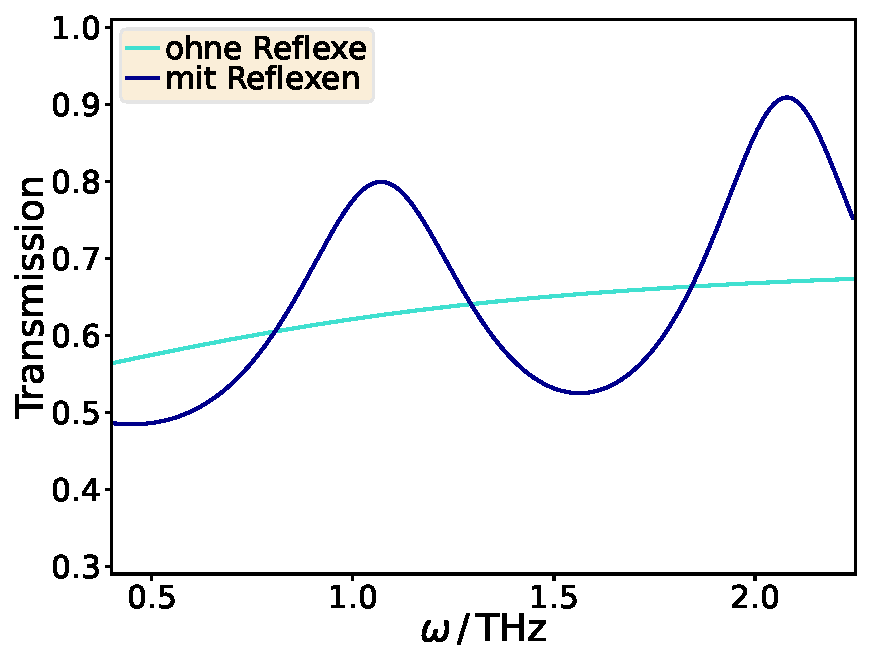
\includegraphics[width=0.6\textwidth]{reflex.pdf}
    \caption{\label{fig:reflex}Vergleich der über das Drude-Modell theoretisch 
    berechneten betraglichen Transmission mit und ohne Berücksichtigung des Etalon-Effekts.}
\end{figure} \FloatBarrier \,\\

\textbf{\textit{Berechnen Sie mit Gl. 3.1 die THz-Transmission T($\mathbf{\omega}$) durch HR-Silizium. Wird
das restliche Licht zum Großteil reflektiert oder absorbiert?}}\\
$\rightarrow$Mit $n_{\text{Si}}=3,4175$ und $n_{\text{Luft}}=1$ folgt
\begin{equation}
    \fbox{$T_{\text{theo}}(\omega) = \frac{4}{n_{\text{Si}}^{2}} \approx 0,7005$}.
\end{equation}
Das restliche Licht wird zum Großteil reflektiert, da aufgrund der hohen Resistivität keine 
Schwingung der Elektronen stattfindet und somit keine Energie absorbiert werden kann. 
Zudem wird mit einem realen Brechungsindex gerechnet, wodurch mathematisch 
keinerlei Reflektion stattfindet \cite{EPC}. 
